\chapter[MapReduce: An Elephant's Perspective]{MapReduce: An Elephant's Perspective}
\label{ch:hadoop}

In this chapter, we review the MapReduce programming
model~\cite{mapreduce-osdi} and the Hadoop system~\cite{hadoop} --- an
open-source software framework that supports data-intensive distributed
applications.  We focus on those aspects of the Hadoop system kernel that
concern the remaining chapters of this thesis.  We begin in
Chapter~\ref{ch:hadoop:sec:progmodel} with the MapReduce programming model,
which is based on two operations; {\em map} and {\em reduce}.  In
Chapter~\ref{ch:hadoop:sec:hadoop}, we present an overview of Hadoop; a system
inspired by Google's MapReduce~\cite{mapreduce-osdi} and the Google File System
(GFS)~\cite{gfs-sosp}.  We conclude in Chapter~\ref{ch:hadoop:sec:conclude} by
introducing our own work in this area, which is further described in the
remaining chapters of this thesis.

\section{MapReduce Programming Model}
\label{ch:hadoop:sec:progmodel}

In MapReduce, the programmer expresses their desired computation as a series of
\emph{jobs} that will yield data in the form of key-value pairs.  Each job
consists of two stages: first, a user-defined \emph{map} function is applied to
each input record to produce a list of intermediate key-value pairs.  Second, a
user-defined \emph{reduce} function is called once for each distinct key in the
map output and passed the list of intermediate values associated with that key.
The MapReduce framework automatically parallelizes the execution of these
functions and ensures fault tolerance.

Optionally, the user can supply a \emph{combiner}
function~\cite{mapreduce-osdi}, which will be applied to the intermediate results
between the map and reduce steps.  Combiners are similar to reduce functions,
except that they are not passed \emph{all} the values for a given key: instead,
a combiner emits an output value that summarizes the input values it was
passed.  Combiners are typically used to perform map-side ``pre-aggregation,''
which reduces the amount of network traffic required between the map and reduce
steps.

\section{Hadoop MapReduce}
\label{ch:hadoop:sec:hadoop}

Hadoop is composed of \emph{Hadoop MapReduce}, an implementation of MapReduce
designed for large clusters, and the \emph{Hadoop Distributed File System}
(HDFS), a file system optimized for batch-oriented workloads such as MapReduce.
In most Hadoop jobs, HDFS is used to store both the input to the map step and
the output of the reduce step.  Note that HDFS is \emph{not} used to store
intermediate results (e.g., the output of the map step): these are kept on each
node's local file system.

A Hadoop installation consists of a single master node and many worker nodes.
The master, called the \emph{JobTracker}, is responsible for accepting jobs
from clients, dividing those jobs into \emph{tasks}, and assigning those tasks
to be executed by worker nodes.  Each worker runs a \emph{TaskTracker} process
that manages the execution of the tasks currently assigned to that node.  Each
{\TT} has a fixed number of slots for executing tasks (two maps and two reduces
by default).  A heartbeat protocol between each {\TT} and the {\JT} is used to
update the {\JT}'s bookkeeping of the state of running tasks, and drive the
scheduling of new tasks: if the \JT identifies free {\TT} slots, it will
schedule further tasks on the {\TT}.

\subsection{Map Task Execution}
\label{ch:hadoop:sec:maptask}

\begin{figure*}[t]
\ssp
\begin{minipage}{\linewidth}
\centering
\begin{verbatim}
public interface Mapper<K1, V1, K2, V2> {
  
  void map(K1 key, V1 value, OutputCollector<K2, V2> output);

  void close();
}
\end{verbatim}
\end{minipage}
\caption{Map function interface (Hadoop version 18.2).}
\label{fig:mapfunction}
\end{figure*}

Each map task is assigned a portion of the input file called a \emph{split}.
By default, a split contains a single HDFS block (64MB by default), so the
total number of file blocks determines the number of map tasks.

The execution of a map task is divided into two phases.
\begin{enumerate}
\item
  The \emph{map} phase reads the task's split from HDFS, parses it into
  records (key/value pairs), and applies the map function to each
  record.
\item
  After the map function has been applied to each input record, the
  \emph{commit} phase registers the final output with the {\TT}, which
  then informs the {\JT} that the task has finished executing.
\end{enumerate}

Figure~\ref{fig:mapfunction} contains the interface that must be implemented by
user-defined map functions.  After the \emph{map} function has been applied to
each record in the split, the \emph{close} method is invoked.  The third
argument to the \emph{map} method specifies an \emph{OutputCollector} instance,
which accumulates the output records produced by the map function.  The output
of the map step is consumed by the reduce step, so the OutputCollector stores
map output in a format that is easy for reduce tasks to consume.  Intermediate
keys are assigned to reducers by applying a partitioning function, so the
OutputCollector applies that function to each key produced by the map function,
and stores each record and partition number in an in-memory buffer.  The
OutputCollector spills this buffer to disk when it reaches capacity.

A spill of the in-memory buffer involves first sorting the records in the
buffer by partition number and then by key.  The buffer content is written to
the local file system as an index file and a data file
(Figure~\ref{ch:hadoop:fig:mapoutput}).  The index file points to the offset of
each partition in the data file.  The data file contains only the records,
which are sorted by the key within each partition segment.

During the \emph{commit} phase, the final output of the map task is generated
by merging all the spill files produced by this task into a single pair of data
and index files.  These files are registered with the {\TT} before the task
completes.  The \TT will read these files when servicing requests from reduce
tasks.

\begin{figure}[t]
  \ssp
  \centering
  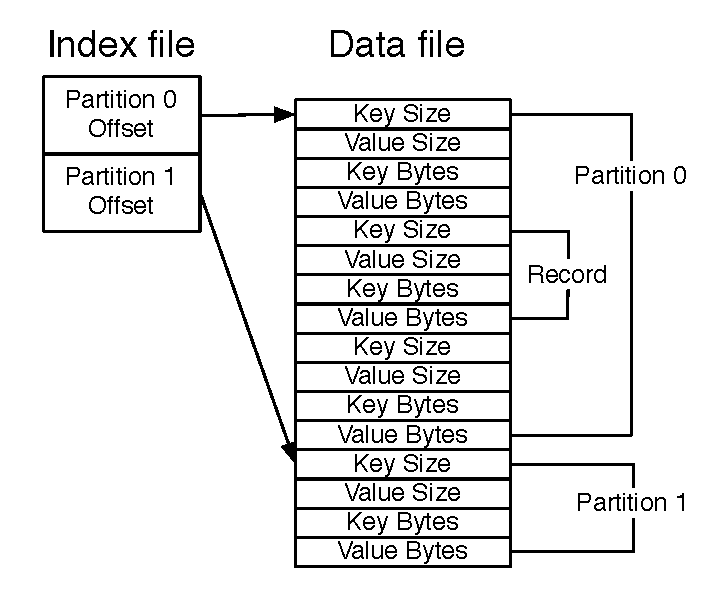
\includegraphics[scale=0.8]{figures/spill_file.pdf}
  \caption{Map task index and data file format (2 partition/reduce case).}
  \label{ch:hadoop:fig:mapoutput}
\end{figure}

\subsection{Reduce Task Execution}
\label{ch:hadoop:sec:reducetask}
The execution of a reduce task is divided into three phases.
\begin{enumerate}
\item The \emph{shuffle} phase fetches the reduce task's input
  data. Each reduce task is assigned a partition of the key range
  produced by the map step, so the reduce task must fetch the content
  of this partition from every map task's output.
\item The \emph{sort} phase groups records with the same key together.
\item The \emph{reduce} phase applies the user-defined reduce function
  to each key and corresponding list of values.
\end{enumerate}

In the \emph{shuffle} phase, a reduce task fetches data from each map task by
issuing HTTP requests to a configurable number of {\TT}s at once (5 by
default). The {\JT} relays the location of every {\TT} that hosts map output to
every {\TT} that is executing a reduce task. Note that a reduce task cannot
fetch the output of a map task until the map has finished executing and
committed its final output to disk.

\begin{figure*}[t]
\ssp
\begin{minipage}{\linewidth}
\begin{verbatim}
public interface Reducer<K2, V2, K3, V3> {

  void reduce(K2 key, Iterator<V2> values, OutputCollector<K3, V3> output);

  void close();
}
\end{verbatim}

\end{minipage}
\caption{Reduce function interface (Hadoop version 18.2).}
\label{fig:reducefunction}
\end{figure*}

After receiving its partition from all map outputs, the reduce task enters the
\emph{sort} phase. The map output for each partition is already sorted by the
reduce key. The reduce task merges these runs together to produce a single run
that is sorted by key. The task then enters the \emph{reduce} phase, in which it
invokes the user-defined reduce function for each distinct key in sorted order,
passing it the associated list of values. The output of the reduce function is
written to a temporary location on HDFS\@. After the reduce function has been
applied to each key in the reduce task's partition, the task's HDFS output file
is atomically renamed from its temporary location to its final location.

In this design, the output of both map and reduce tasks is written to disk
before it can be consumed. This is particularly expensive for reduce tasks,
because their output is written to HDFS\@. Output materialization simplifies
fault tolerance, because it reduces the amount of state that must be restored to
consistency after a node failure. If any task (either map or reduce) fails, the
{\JT} simply schedules a new task to perform the same work as the failed
task. Since a task never exports any data other than its final answer, no
further recovery steps are needed.

 % Mention fault-tolerance/atomic
% rename here?

% \subsection{Dataflow in Hadoop}
% Hadoop \emph{materializes} the output of the map and reduce functions
% in two places:

% \begin{itemize}
% \item
%   Between the map and reduce steps, the output of each map task is
%   written to disk before it can be read by any reduce tasks.
% \item
%   The output of the reduce step is written to HDFS at the end of each
%   job. As we observed in Section~\ref{sec:progmodel}, many practical
%   computations are written as a chain of MapReduce computations
%   (e.g.\ PageRank). In that setting, writing the output of each job to
%   HDFS and then reading it back again is inefficient.
% \end{itemize}



\section{Summary}
\label{ch:hadoop:sec:conclude}

The MapReduce interface is a good example of capturing the minimum essentials
of an abstraction, making it easy to build many higher-order constructs (e.g.,
data analysis~\cite{pig-sigmod}, SQL~\cite{hive-vldb}, machine
learning~\cite{mahout}) while allowing significant flexibility in the system
implementation.  Fault-tolerance was an early part of the MapReduce system
design, and one of its most attractive features.  The fault-tolerance model is
predicated on the batch-oriented nature of MapReduce, allowing the recovery of
a task to simply be restarting it on some (possibly alternate) machine.  Since
no state, in the form of output data, is allowed to exit a task (map or
reduce), no further recovery actions are required.

Optimization at the MapReduce level often comes in the form of scheduling
policies that primarily focus on job response time.  The runtime of a MapReduce
job is determined by its slowest tasks.  The slowest map task determines the
finishing time of the {\em shuffle} phase since reduce tasks are not able to
enter the {\em reduce} phase until they have received all the map outputs that
belong to them.  The slowest reduce task determines the finishing time of the
overall job since a job does not complete until all reduce tasks complete.
Speculation is a response-time optimization that executes clones of tasks
deemed to be slow.  Alternative speculation policies for identifying and
speculatively scheduling these 'straggler' tasks exist~\cite{mapreduce-osdi,
zaharia-late}, but there is no consensus on a policy that works well for all
jobs and cluster configurations.

In Chapter~\ref{ch:boom}, we describe an implementation of the Hadoop MapReduce
engine in the \OVERLOG language.  This declarative specification of Hadoop
enables us to build alternative scheduling policies and optimizations in a high
level query language improving the development cycle and decreasing the lines
of code by {\em orders of magnitude}, all while supporting a richer suite of
scheduling strategies.  In Chapter~\ref{ch:hop}, we move from a batch-oriented
execution model to a pipelined model where tasks incrementally send their
output.  Pipelining enables two new features in the context of MapReduce:
online aggregation~\cite{onlineagg} and continuous queries.  We show that a
pipelined implementation of MapReduce does not sacrifice the original system
interface or its ability to tolerate faults.  A pipelined MapReduce model
extends the range of scheduling alternatives, which we easily support through
policies written in \OVERLOG.

